\begin{frame}{Polygon with Measurements}
\begin{center}
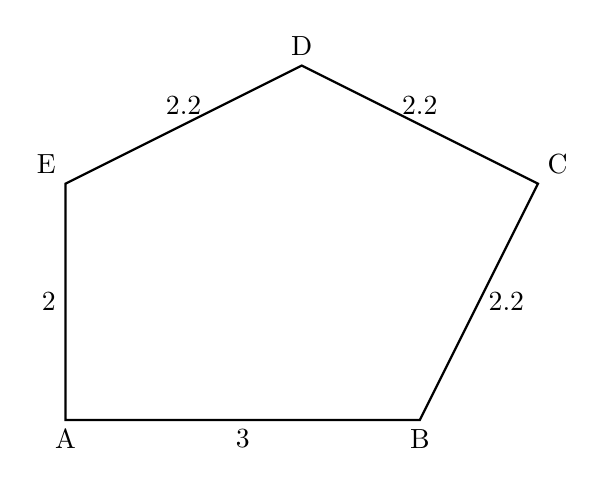
\begin{tikzpicture}[scale=1.5]
    \draw[thick] (0,0) -- (3,0) -- (4,2) -- (2,3) -- (0,2) -- cycle;
    \node[below] at (0,0) {A};
    \node[below] at (3,0) {B};
    \node[above right] at (4,2) {C};
    \node[above] at (2,3) {D};
    \node[above left] at (0,2) {E};
    
    % Side measurements
    \node[below] at (1.5,0) {3};
    \node[right] at (3.5,1) {2.2};
    \node[above] at (3,2.5) {2.2};
    \node[above] at (1,2.5) {2.2};
    \node[left] at (0,1) {2};
\end{tikzpicture}
\end{center}

\footnotesize
Irregular pentagon with labeled vertices and side lengths
\end{frame}